\section{\no Minimum-Size Slicing}
\label{sec:complexity}

\sectionlegend

We can calculate a \textit{minimal} synthesis slice in polynomial time (\cref{sec:min-exists}). However, minimal slices are not unique, so a natural extension is to rank them by \textit{size} and ask for a minimal slice of \textit{minimum size}. This chapter reduces the \textit{set cover optimisation problem} to calculating minimum size slice, meaning minimum-size slicing is \textbf{NP-hard}. I (informally) prove this for term-minimal synthesis slices, and show that the argument extends to general minimal synthesis slices and to analysis slices.

\subsection{\no Definitions}\label{sec:complexity-setup}

\begin{definition}[Size of an Expression Slice]\label{def:slice-size}
For an expression slice $\varsigma \in \lfloor e \rfloor$, the size $|\varsigma|$ counts non-$\gap$ syntactic positions:
\[
  |\gap| = 0,\qquad |*| = 1,\qquad |x| = 1, \qquad |c(\varsigma_1, \dots, \varsigma_k)| = 1 + \textstyle\sum_i |\varsigma_i|.
\]
\end{definition}

\begin{definition}[\textsc{Minimum-Size TermMinimal Slice Problem}]\label{def:min-tm-slice}
Given a derivation $D : \synthesis{e}{\tau}$ and query $\upsilon \in \lfloor\tau\rfloor$, the minimum-size term-minimal slice problem is to compute
\[
  \mathrm{minSize}(D, \upsilon) \;\triangleq\; \min\bigl\{\,|\sigma| \;:\; \sigma \in \tmslice{D}{\upsilon}\,\bigr\}.
\]
\end{definition}

\begin{definition}[\textsc{Minimum Set Cover (Optimisation) Problem}]\label{def:min-set-cover}
Given a universe $U = \{1, \dots, n\}$ and a family $S = S_1, \dots, S_m \subseteq U$, compute
\[
  K^\star(U, S) \;\triangleq\; \min\bigl\{\,|J| \;:\; J \subseteq \{1, \cdots, m\},\; \textstyle\bigcup_{j \in J} S_j = U\,\bigr\}.
\]
\end{definition}

The minimum set cover optimisation problem is NP-hard~\cite[\S16.1, p.~414]{KorteVygen}, hence any polynomial reduction from it, is also NP-hard.

\subsection{\no The reduction}\label{sec:complexity-reduction}

\begin{definition}[Reduction to Min-set-cover]\label{def:reduction}
Given an instance $(U, S_1, \dots, S_m)$ of \textsc{Min-Set-Cover}, suppose wlog. $|U| = n$ and $\bigcup_j S_j = U$. Then construct $D : \synthesis{e}{\tau}$ and query $\upsilon = \tau$ as follows:
\begin{itemize}
\item \textbf{Target type $\tau$:} $\tau \;=\; \underbrace{*\,\times\,(*\,\times\,(\cdots \times (*\,\times\,*)))}_{n \text{ projections}}$. Position $i$ of $\tau$ corresponds to element $i$ of $U$.
\item \textbf{Encoding $S_j \mapsto T_j$:} For each $j$, construct type slice family $T_j \in \lfloor\tau\rfloor$ by omitting all projections $i$ for $i \not\in S_j$. Then $\bigsqcup_{j} T_j = \tau$ iff $\bigcup_j S_j = U$, where $\bigsqcup_j$ is the finite join of family $T_j$.
\item \textbf{Assumption context $\Gamma$:} $\Gamma \;=\; (x_1 : T_1,\; \dots,\; x_m : T_m)$, so each $x_j$ synthesises $T_j$ exactly under \synr{Var}.
\item \textbf{Case tree $e$:} Construct any binary case tree with leaves $x_1, \dots, x_m$, and having all scrutiness being $\gap$ and all binders being $x$.

By \cref{lem:slices-consistent} the leaves' synthesised types are mutually consistent, so the case rule applies at every node, giving $\synthesis{e}{\bigsqcup_j T_j} = \synthesis{e}{\tau}$. The tree has size $|e| = 2m - 1$: $m$ leaves and $m-1$ case expressions.
\item \textbf{Query:} $\upsilon = \tau$.
\end{itemize}
\end{definition}

\noindent This construction is trivially computable in polynomial (linear) time: $\mathcal{O}(n + m + \sum_{j}{|S_j|}).$

Concretely, view each set $S_j$ as a \textit{variable} $x_j$ whose type is a slice of the target carrying $*$ exactly where $S_j$ has an element. Then any slice of the case tree $e$ represents a choice of variables $x_j$. \Cref{fig:set-cover-case-tree} draws this correspondence on a $4$-element universe.

\begin{figure}[ht]
\centering
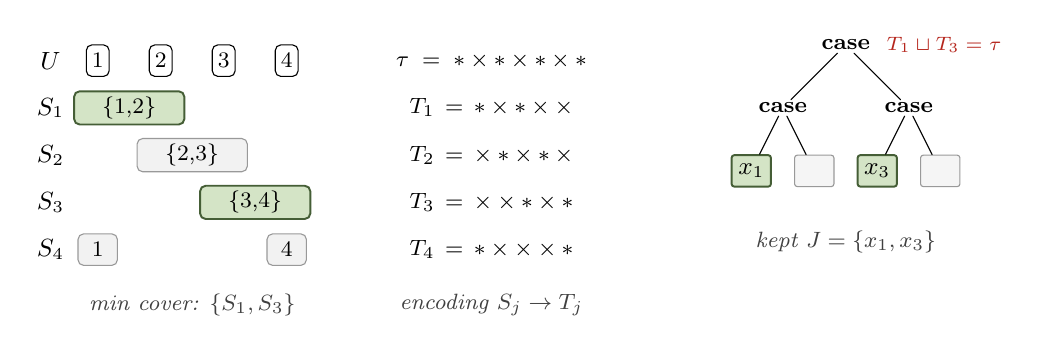
\begin{tikzpicture}[
    sc/.style={draw, rounded corners=2pt, inner sep=2pt, minimum height=4mm, font=\footnotesize},
    sel/.style={fill=OliveGreen!18, draw=OliveGreen!60!black, line width=0.7pt},
    no/.style={fill=black!5, draw=black!40},
    ca/.style={font=\bfseries\footnotesize, inner sep=1pt},
    lf/.style={draw, rounded corners=1pt, inner sep=2pt, minimum width=5mm, minimum height=4mm, font=\small},
    kp/.style={draw=OliveGreen!60!black, fill=OliveGreen!18, line width=0.7pt},
    dr/.style={draw=black!40, fill=black!4, text=black!50},
    every node/.append style={font=\small},
    line cap=round]

\node[font=\itshape\small] at (-0.6,0.6) {$U$};
\node[sc] at (0.0,0.6) {1};
\node[sc] at (0.8,0.6) {2};
\node[sc] at (1.6,0.6) {3};
\node[sc] at (2.4,0.6) {4};

\node[font=\itshape\small] at (-0.6,0.0) {$S_1$};
\node[sc, sel, minimum width=14mm] at (0.4,0.0) {\{1,2\}};
\node[font=\itshape\small] at (-0.6,-0.6) {$S_2$};
\node[sc, no,  minimum width=14mm] at (1.2,-0.6) {\{2,3\}};
\node[font=\itshape\small] at (-0.6,-1.2) {$S_3$};
\node[sc, sel, minimum width=14mm] at (2.0,-1.2) {\{3,4\}};
\node[font=\itshape\small] at (-0.6,-1.8) {$S_4$};
\node[sc, no,  minimum width=5mm]  at (0.0,-1.8) {1};
\node[sc, no,  minimum width=5mm]  at (2.4,-1.8) {4};

\node[font=\footnotesize\itshape, text=gray!50!black, align=center] at (1.2,-2.5)
  {min cover: $\{S_1,S_3\}$};

\node[font=\footnotesize, align=left] at (5.0,0.6)  {$\tau \;=\; * \times * \times * \times *$};
\node[font=\footnotesize, align=left] at (5.0,0.0)  {$T_1 \,=\, * \times * \times \gap \times \gap$};
\node[font=\footnotesize, align=left] at (5.0,-0.6) {$T_2 \,=\, \gap \times * \times * \times \gap$};
\node[font=\footnotesize, align=left] at (5.0,-1.2) {$T_3 \,=\, \gap \times \gap \times * \times *$};
\node[font=\footnotesize, align=left] at (5.0,-1.8) {$T_4 \,=\, * \times \gap \times \gap \times *$};
\node[font=\footnotesize\itshape, text=gray!50!black, align=center] at (5.0,-2.5)
  {encoding $S_j \to T_j$};

\node[ca] (rt) at (9.5, 0.8) {case};
\node[ca] (cl) at (8.7, 0.0) {case};
\node[ca] (cr) at (10.3,0.0) {case};
\node[lf, kp] (l1) at (8.3,-0.8) {$x_1$};
\node[lf, dr] (l2) at (9.1,-0.8) {$\gap$};
\node[lf, kp] (l3) at (9.9,-0.8) {$x_3$};
\node[lf, dr] (l4) at (10.7,-0.8) {$\gap$};
\draw (rt) -- (cl);
\draw (rt) -- (cr);
\draw (cl) -- (l1);
\draw (cl) -- (l2);
\draw (cr) -- (l3);
\draw (cr) -- (l4);
\node[font=\scriptsize, text=BrickRed, anchor=west] at (rt.east) {\,$T_1 \sqcup T_3 = \tau$};
\node[font=\footnotesize\itshape, text=gray!50!black, align=center] at (9.5,-1.7)
  {kept $J = \{x_1, x_3\}$};

\end{tikzpicture}
\caption{Set cover (left), the encoding (middle), and the induced case-tree slice (right), with a minimal set cover selected.}
\label{fig:set-cover-case-tree}
\end{figure}

\subsection{\no Correctness}\label{sec:complexity-correctness}

Throughout this subsection, write $J(\sigma) = \{j : x_j \in \varsigma\}$ for the set of leaves retained in a slice $\sigma$ of $e$.

\begin{lemma}[Validity is Set-Cover]\label{lem:tm-validity}
A term-minimal slice $\sigma$ of $D$ at $\upsilon = \tau$ is valid iff $J(\sigma)$ is a set cover of $U$.
\end{lemma}

\begin{proof}
Under fixed $\Gamma$, $x_j$ in the slice synthesises $T_j$ (rule \synr{Var}), and a $\gap$-leaf synthesises $\gap$. Walking up the case tree, the case rule joins branch types pointwise, so $\sigma$ synthesises $\bigsqcup_{j \in J(\sigma)} T_j$. Validity ($\sqsupseteq \tau$) holds iff every position of $\tau$ is covered. As $\tau$ encodes $U$, then validity holds iff $\bigcup_{j \in J(\sigma)} S_j = U$.
\end{proof}

\begin{lemma}[Minimum Set Size]\label{lem:tm-size}
For $(\Gamma, e, \tau)$ encoding Min-Set-Cover problem $(U, S)$. From minSize$(\synthesis{e}{\tau}, \tau)$ we can calculate $K^{\star}(U, S)$ in polynomial time.
\end{lemma}

\begin{proof}
Recurse once through minSize$(\synthesis{e}{\tau}, \tau)$ and count the number of variables, this is $|J(\sigma)| = K^{\star}(U,S)$. As $\sigma \sqsubseteq e$, then $|\sigma| \leq |e| = 2m - 1$, hence time complexity of this is $\mathcal{O}(m)$.
\end{proof}

\begin{majortheorembox}
\begin{theorem}[\textsc{Minimum-Size Term-Minimal-Slicing} is NP-hard]\label{thm:tm-min-nph}
Computing $\mathrm{minSize}(D, \upsilon)$ is NP-hard.
\end{theorem}
\end{majortheorembox}

\begin{proof}
Definition~\ref{def:reduction} is a polynomial-time many-one reduction from \textsc{Min-Set-Cover} to \textsc{Min-TM-Slice}, and Lemma~\ref{lem:tm-size} recovers $K^\star(U, S)$ from $\mathrm{minSize}(D, \upsilon)$ in polynomial time. Hence \textsc{Min-Set-Cover} $\le_p$ \textsc{Min-TM-Slice}, and NP-hardness of \textsc{Min-Set-Cover}~\cite[\S16.1, p.~414]{KorteVygen} transfers.
\end{proof}

\subsection{\no Extension to Min-Syn-Slice}\label{sec:min-syn-extension}

The reduction above can be embedded also into minimum synthesis slices, by forcing the minimal assumptions slice to be full by producting the case tree with all the variables $x_j$ and querying each set in this product fully.

\begin{definition}[Reduction to Min-Syn-Slice]\label{def:syn-reduction}
Let $(\Gamma, e_0, \tau)$ be the term-minimal encoding of Definition~\ref{def:reduction}. Form the product expression and query
\[
  e \;\triangleq\; (e_0,\, x_1,\, x_2,\, \dots,\, x_m),
  \qquad
  \upsilon \;\triangleq\; \tau \times T_1 \times T_2 \times \cdots \times T_m,
\]
under the same assumption context $\Gamma = (x_1 : T_1, \dots, x_m : T_m)$.
\end{definition}

\begin{lemma}[Maximal Assumption Slice]\label{lem:forced-gamma}
For every valid slice $\rho = (\gamma, \varsigma)$ of $\synthesis{e}{\upsilon}$ at $\upsilon$, $\gamma = \Gamma$.
\end{lemma}

\begin{proof}
The $(j+1)$-th projection is $x_j$ and is queried at $T_j$. This projection must synthesise $T_j$ under $\gamma$ via \synr{Var}. Hence, we require $\gamma(x_j) = T_j$, so $\gamma = \Gamma$.
\end{proof}

\begin{majortheorembox}
\begin{theorem}[\textsc{Minimum-Size Syn-Slice} is NP-hard]\label{thm:syn-min-nph}
Computing $\min\{|\rho| : \rho \in \synslice{D}{\upsilon}\}$ is NP-hard.
\end{theorem}
\end{majortheorembox}

\begin{proof}
By Lemma~\ref{lem:forced-gamma}, $|\gamma| = |\Gamma|$ is fixed by the input, and the outer-tuple variable positions $x_1, \dots, x_m$ contribute a further fixed $m$. Hence $|\rho| = |\Gamma| + m + |\varsigma_0|$, where $\varsigma_0$ slices the case-tree component $e_0$, and minimising $|\rho|$ reduces to the term-minimal problem on $(e_0, \tau)$. The construction is polynomial in $n + m$, and NP-hardness transfers from Theorem~\ref{thm:tm-min-nph}.
\end{proof}

%%% Local Variables:
%%% mode: LaTeX
%%% TeX-master: "PolymorphicTypeSlicing"
%%% End:
